% !TeX program = lualatex
% !BIB program = biber
% Lualatex is important to render TTF fonts; with pdflatex it's just the regular one
% ratio 16:9 -- https://tex.stackexchange.com/questions/14336/

% compile two versions, inspired by https://tex.stackexchange.com/a/1501
% use the script "compile-pdf.sh"
\newif\ifhandout
% if flags.tex does not exist, create an empty file to be able to compile in TeXstudio
\input{flags}

\ifhandout
\documentclass[12pt,aspectratio=169,handout]{beamer}
\else
\documentclass[12pt,aspectratio=169]{beamer}
\fi



% TODO change "leftfootertext" to your liking
\newcommand{\leftfootertext}{\insertsubtitle}  % just the \title{} text by default
%\newcommand{\leftfootertext}{RNNs and encoder-decoder architectures}  % Your name, for instance


% ------- RUB specifics ----------
% adjust for 16:9
% https://tex.stackexchange.com/questions/354022/modifying-the-margins-of-all-slides-in-beamer
\setbeamersize{text margin left=0.3cm,text margin right=4.5cm} 


% use Metropolis as the basis theme
\usetheme[subsectionpage=progressbar]{metropolis}
% blocks with background globally
\metroset{block=fill}


\usepackage{fontspec}
% RUB fonts need to be installed
% 'UprightFont = * Light' makes sure that the base font is RubFlama Light, which looks
% lighter than RubFlama Regular (would be too thick for slides)
\setsansfont[Scale=MatchLowercase, UprightFont = * Light, BoldFont = * Bold]{RubFlama}
%\setsansfont{Arial} % Open source alternative if you don't have RubFlama

% RUB color scheme
% Dark blue: 0; 53; 96; #003560
\definecolor{RUBDarkBlue}{RGB}{0, 53, 96}

% Light yellow (table fill, etc.); 238; 250; 196; #EEFAC4
\definecolor{RUBLightYellow}{RGB}{238, 250, 196}

%Light green: 141; 174; 16
\definecolor{RUBLightGreen}{RGB}{141, 174, 16}


\setbeamercolor{titlelike}{fg=RUBDarkBlue}
\setbeamercolor{subtitle}{fg=RUBLightGreen}
\setbeamercolor{separation line}{fg=RUBLightGreen}
\setbeamercolor{frametitle}{bg=white, fg=RUBDarkBlue}

% horizontal line on title page and sections
\setbeamercolor{alerted text}{fg=RUBLightGreen}


% Adjust footer bottom (too large by default)
\setbeamertemplate{footline}{%
  \begin{beamercolorbox}[wd=\textwidth, sep=2ex]{footline}%
    \usebeamerfont{page number in head/foot}%
    \usebeamertemplate*{frame footer}
    \hfill%
    \usebeamertemplate*{frame numbering}
  \end{beamercolorbox}%
}


% Lab name, numbering, etc. in footer
\setbeamertemplate{frame numbering}{TrustHLT --- Prof.\ Dr.\ Ivan Habernal \hspace*{1ex} 
\includegraphics[width=7em]{img/rub-logo.pdf}\hspace*{1ex}}

\setbeamertemplate{frame footer}{\hspace*{1ex}\insertframenumber \hspace*{2ex} \leftfootertext}

% adjust the background to be completely white
\setbeamercolor{background canvas}{bg=white}

% logos on the title page
\titlegraphic{%
	\begin{picture}(0,0)
		\put(435,0){\makebox(0,0)[rt]{
\includegraphics[width=7em]{img/rub-logo.pdf}}}
		\put(435,-170){\makebox(0,0)[rt]{
\includegraphics[width=4em]{img/logo-trusthlt.pdf}}}
		\put(435,-196){\makebox(0,0)[rt]{
\includegraphics[width=9em]{img/logo-rctrust.pdf}}}
	\end{picture}%
}


% show TOC at every section start
\AtBeginSection{
	\frame{
		\vspace{2em}
		\sectionpage
		\hspace*{2.2em}\begin{minipage}{10cm}
			\tableofcontents[currentsection]
		\end{minipage}
	}
}

% TOC without subsection
\setcounter{tocdepth}{1} % only-- part,chapters,sections 

% bullet points: rectangles
\useinnertheme{rectangles}
\setbeamercolor{itemize item}{fg=RUBLightGreen}
\setbeamercolor{itemize subitem}{fg=RUBLightGreen}
% enumerate: blue background for better readability
\setbeamercolor{item projected}{bg=RUBDarkBlue}

% make boxes (example, block, etc.) background lighter for readability
\setbeamercolor{block title}{%
	use=normal text,
	fg=normal text.fg,
	bg=normal text.bg!90!fg % lighter background in block title
}
\setbeamercolor{block body}{
	use={block title, normal text},
	bg=block title.bg!30!normal text.bg % lighter background in block body
}


% RUB colors in blocks
\setbeamercolor{block title alerted}{%
	use={block title, alerted text},
	bg=RUBDarkBlue,
	%fg=RUBLightYellow % looks bad
	fg=white % better contrast
}

\setbeamercolor{block title example}{%
	use={block title, example text},
	fg=RUBLightGreen
}


% ------- end of RUB specifics ----------

% all itemize with pause by default
%\beamerdefaultoverlayspecification{<+->}


% typeset mathematics on serif
\usefonttheme[onlymath]{serif}

% better bibliography using biber as backend
\usepackage[natbib=true,backend=biber,style=authoryear-icomp,maxbibnames=30,maxcitenames=9,uniquelist=false,giveninits=true,doi=false,url=false,dashed=false,isbn=false]{biblatex}
% shared bibliography
\addbibresource{../bibliography.bib}
% disable "ibid" for repeated citations
\boolfalse{citetracker}



\usepackage{xspace}


% for derivatives, https://tex.stackexchange.com/a/412442
\usepackage{physics}

\usepackage{tikz}
\usetikzlibrary{matrix, positioning}
\usetikzlibrary{angles,quotes} % for angles
\usetikzlibrary{backgrounds} % background
\usetikzlibrary{decorations.pathreplacing} % curly braces
\usetikzlibrary{calligraphy}
\usetikzlibrary{calc} % for neural nets

% for plotting functions
\usepackage{pgfplots}
\usepgfplotslibrary{dateplot}

% sub-figures
\usepackage{caption}
\usepackage{subcaption}

% book tabs
\usepackage{booktabs}


% argmin, argmax
\usepackage{amsmath}
\DeclareMathOperator*{\argmax}{arg\!\max}
\DeclareMathOperator*{\argmin}{arg\!\min}
% softmax
\DeclareMathOperator*{\softmax}{soft\!\max}
% Mask
\DeclareMathOperator*{\mask}{mask}

% bold math
\usepackage{bm}

% for \mathclap
\usepackage{mathtools}

% algorithms
\usepackage[noend]{algpseudocode}


% for neurons and layers in tikz
\tikzset{
	neuron/.style={draw, rectangle, inner sep=2pt, minimum width=0.75cm, fill=blue!20},
	param/.style={draw, rectangle, inner sep=2pt, minimum width=0.75cm, fill=green!20},
	constant/.style={draw, rectangle, inner sep=2pt, minimum width=0.75cm, fill=black!15},
	% for citation nodes right top
	ref/.style={anchor = north east, text width=7.8cm, yshift=-1.3cm, xshift=-0.2cm, scale=0.5},
	state/.style={rectangle, inner sep=2pt, minimum width=0.75cm, fill=black!5},
}

% added in lecture 10
\tikzset{
	mtx/.style={
		matrix of math nodes,
		left delimiter={[}, right delimiter={]}
	},
	hlt/.style={opacity=0.1, line width=4 mm, line cap=round},
	hltr/.style={opacity=0.5, rounded corners=2pt, inner sep=-1pt}
}

% for strike-through text (added in Lecture 06)
\usepackage[normalem]{ulem}

% added in Lecture 7
% RNN
\DeclareMathOperator*{\rnn}{RNN}
% RNN star
\DeclareMathOperator*{\rnnstar}{RNN^{*}}
% bi-RNN
\DeclareMathOperator*{\birnn}{biRNN}


% added in Lecture 9
\usetikzlibrary{fit} % for hightligting by calling "fit"

% algorithms
\usepackage[noend]{algpseudocode}



\title{Privacy-Preserving Natural Language Processing}
\subtitle{Lecture 3 -- Introduction to Differential Privacy}
\date{April 24, 2025}
\author{Prof.\ Dr.\ Ivan Habernal}
\institute{
\texttt{www.trusthlt.org} \\
Chair of Trustworthy Human Language Technologies (TrustHLT) \\
Ruhr University Bochum \& Research Center Trustworthy Data Science and Security}

\begin{document}

\maketitle


\section{Intro}

\begin{frame}{Overview}

First lecture: privacy definitions, arbitrary hard choices

Second lectures: still arbitrary choice in anonymization, but GDPR notion of possibility of deidentification

Today: towards probabilistic approach to privacy


%\begin{tikzpicture}[overlay, remember picture]
%\node at (current page.north east)[ref] {
%\fullcite{Voigt.Bussche.2017} \par};
%\end{tikzpicture}
\end{frame}


\section{Differential privacy basics}



\begin{frame}{Precursors of differential privacy}

"Let us begin with a short story. Envision a database of a hospital containing the medical history of some population. On one hand, the hospital would like to advance medical research which is based (among other things) on statistics of the information in the database. On the other hand, the hospital is obliged to keep the privacy of its patients, i.e. leak no medical information that could be related to a specific patient. The hospital needs an access mechanism to the database that allows certain ‘statistical’ queries to be answered, as long as they do not violate the privacy of any single patient."


\begin{tikzpicture}[overlay, remember picture]
\node at (current page.north east)[ref] {
\fullcite{dinurRevealingInformationPreserving2003} \par};
\end{tikzpicture}
\end{frame}



\begin{frame}{Precursors of differential privacy}

"We focus on binary databases, where the content is of $n$ binary (0-1) entries"


\begin{tikzpicture}[overlay, remember picture]
\node at (current page.north east)[ref] {
\fullcite{dinurRevealingInformationPreserving2003} \par};
\end{tikzpicture}
\end{frame}



\begin{frame}{First DP papers}

"The database consists of some number $n$ of rows. We are completely agnostic about the type of rows – they may be tuples of attributes, strings, or even pictures."

\begin{tikzpicture}[overlay, remember picture]
\node at (current page.north east)[ref] {
\fullcite{blumPracticalPrivacySuLQ2005} \par};
\end{tikzpicture}
\end{frame}


\begin{frame}{Explicit notion of independence of rows}


\begin{block}{Dependency Between Database Records}
``We explicitly assume that the database records are chosen independently from each other, according to some underlying distribution $D$. We are not aware of any work that does not make this assumption (implicitly or explicitly)."
\end{block}


\begin{tikzpicture}[overlay, remember picture]
\node at (current page.north east)[ref] {
\fullcite{Dwork.Nissim.2004.CRYPTO} \par};
\end{tikzpicture}
\end{frame}

\begin{frame}{Explicit notion of independence of rows}


"The intent of the independence assumption is to characterize what information is under the control of a given individual. Specifically, \textbf{if there is information about a row that can be learned from other rows, this information is not truly under the control of that row.} Even if the row in question were to sequester itself away in a high mountaintop cave, information about the row that can be gained from the analysis of other rows is still available to an adversary. It is for this reason that \textbf{we focus our attention on those inferences that can be made about rows without the help of others}."


\begin{tikzpicture}[overlay, remember picture]
\node at (current page.north east)[ref] {
\fullcite{blumPracticalPrivacySuLQ2005} \par};
\end{tikzpicture}
\end{frame}

\section{Dataset}

\begin{frame}{Dataset (or Database)}

\begin{block}{The essential assumption (in words)}
Each person corresponds to a single row in a table
\end{block}

The semantics of columns is arbitrary:

\begin{itemize}
\item It could be an actual "table" with some sensitive attributes (e.g., age, income)
\item It could be just an arbitrary unstructured object (e.g., personal photo, text)
\end{itemize}

%\begin{tikzpicture}[overlay, remember picture]
%\node at (current page.north east)[ref] {
%\fullcite{Voigt.Bussche.2017} \par};
%\end{tikzpicture}
\end{frame}


\begin{frame}{Dataset}

\begin{block}{Another implicit assumption}
Each row contains data (values or attributes) that "belong" to this row's person
\end{block}


\begin{block}{Implication of the above assumption}
Example: If person A is removed from the dataset, you cannot certainly tell her private attributes from some other row B, C, D.
\end{block}



%\begin{tikzpicture}[overlay, remember picture]
%\node at (current page.north east)[ref] {
%\fullcite{Voigt.Bussche.2017} \par};
%\end{tikzpicture}
\end{frame}


\begin{frame}{Examples of implicit assumptions}

\begin{table}
\footnotesize
\begin{tabular}{lrr} \toprule
Name & Income & Age \\ \midrule
Bob & 700 & 21 \\
Alice & 2,800 & 32 \\
Charlie & 3,500 & 45 \\ \bottomrule
\end{tabular}
\caption{Looks legit, no clear violation of the assumptions}
\end{table}

\vspace{-1em}
\begin{table}
\footnotesize
\begin{tabular}{lrrr} \toprule
Name & Income & Age & Someone else's income \\ \midrule
Bob & 700 & 21 & Alice: 2,800\\
Alice & 2,800 & 32 & Charlie: 3,500 \\
Charlie & 3,500 & 45 & Alice: 2,800 \\ \bottomrule
\end{tabular}
\caption{Something looks wrong with this dataset}
\end{table}

%\begin{tikzpicture}[overlay, remember picture]
%\node at (current page.north east)[ref] {
%\fullcite{Voigt.Bussche.2017} \par};
%\end{tikzpicture}
\end{frame}

\begin{frame}{Examples of implicit assumptions}


\begin{table}
\footnotesize
\begin{tabular}{lrr} \toprule
Name & Income & Age \\ \midrule
Bob & 700 & 21 \\
Alice & 2,800 & 32 \\
Charlie & 3,500 & 45 \\
Alice & 2,800 & 32 \\
\bottomrule
\end{tabular}
\caption{Something looks wrong with this dataset}
\end{table}

%\begin{tikzpicture}[overlay, remember picture]
%\node at (current page.north east)[ref] {
%\fullcite{Voigt.Bussche.2017} \par};
%\end{tikzpicture}
\end{frame}



\section{Statistical queries}


\begin{frame}{Real-valued query}

"Trusted server that holds a database of sensitive information. Given a query function $f$ mapping databases to reals, the so-called true answer is the result of applying $f$ to the database. [...]"

\begin{block}{Query}
Let $X$ be a database from a universe (a set) of all possible databases $\mathcal{X}$

Real-valued query is
$$
f: \mathcal{X} \mapsto \mathbb{R}
$$
\end{block}



\begin{tikzpicture}[overlay, remember picture]
\node at (current page.north east)[ref] {
\fullcite{dworkCalibratingNoiseSensitivity2006} \par};
\end{tikzpicture}
\end{frame}



\begin{frame}{Query example -- "counting" query}

"A query consists of a pair $(S, f)$ where $S$ is a set of rows in the database and $f$ is a function mapping database rows to $\{0, 1\}$. The true answer is $\sum_{i \in S} f(d_i)$"

\begin{itemize}
\item implicitly assuming $d_i$ is the $i$-th entry from $S$
\item also note inconsistencies in notations, inevitable in every new field being just formalized!! Here $f$ maps a "row" to zero or one, previous slide $f$ would be the whole sum
\end{itemize}

\begin{tikzpicture}[overlay, remember picture]
\node at (current page.north east)[ref] {
\fullcite{dworkCalibratingNoiseSensitivity2006} \par};
\end{tikzpicture}
\end{frame}


\begin{frame}{How could a counting query leak private information?}

"It's just a statistics (a sum), so I can hide in the crowd!"

\begin{block}{What is private information}
The secret "bit" $f(d_i) \mapsto \{0, 1\}$

which eventually corresponds to whether or not you are in the database
\end{block}


\begin{itemize}
\item If your are in the database, you cannot control others
\item What if the database is very small?
\item What if the database is queried repeatedly?
\item What if you are an outlier?
\end{itemize}




%\begin{tikzpicture}[overlay, remember picture]
%\node at (current page.north east)[ref] {
%\fullcite{Voigt.Bussche.2017} \par};
%\end{tikzpicture}
\end{frame}



\subsection{How to protect privacy in counting queries}


\begin{frame}{Example}

\begin{table}
\footnotesize
\begin{tabular}{lrrr} \toprule
Name & Hospitalized in year & Age & Illegal drug use \\ \midrule
Alice & 2024 & 32 & yes \\
Bob & 2020 & 21 & no \\
Charlie & 2023 & 45 & no \\
$\ldots$ & & & \\
Xander & 2020 & 31 & yes \\ \bottomrule
\end{tabular}
\caption{A sensitive database example from a clinic}
\end{table}

Query: How many persons in the database take illegal drugs?

\begin{tikzpicture}[overlay, remember picture]
\node at (current page.north east)[ref] {
(Important to clarify for context: If you are Alice, how did you end up in such a database?) \par};
\end{tikzpicture}



%\begin{tikzpicture}[overlay, remember picture]
%\node at (current page.north east)[ref] {
%\fullcite{Voigt.Bussche.2017} \par};
%\end{tikzpicture}
\end{frame}


\begin{frame}{Example: How many persons in the database take illegal drugs?}

\begin{table}
\scriptsize
\begin{tabular}{lrrr} \toprule
Name & Hospitalized in year & Age & Illegal drug use \\ \midrule
Alice & 2024 & 32 & yes \\
Bob & 2020 & 21 & no \\
Charlie & 2023 & 45 & no \\
$\ldots$ & & & \\
Xander & 2020 & 31 & yes \\ \bottomrule
\end{tabular}
\end{table}

What might be public information: the size of the dataset (say $n = 100$)

The true answer to the query: 2

If Xander reveals his drug use, and we know Alice is in the database, her privacy is revealed!

%\begin{tikzpicture}[overlay, remember picture]
%\node at (current page.north east)[ref] {
%\fullcite{Voigt.Bussche.2017} \par};
%\end{tikzpicture}
\end{frame}






\subsection{How to protect privacy}


\begin{frame}{Privatizing the query result}

How would you go about it?

%\begin{tikzpicture}[overlay, remember picture]
%\node at (current page.north east)[ref] {
%\fullcite{Voigt.Bussche.2017} \par};
%\end{tikzpicture}
\end{frame}





\begin{frame}{Solution: Alter the query result}

Changes to the true query result must be \textbf{irreversible}!

"A natural approach, and one that has been explored by others in the 1980’s, is to add random noise to the answer" \citep{blumPracticalPrivacySuLQ2005}

"It is evident that without randomness there is no privacy: if everything is pre-determined, and all possible choices we make are predictable or pre-programmed by our adversaries, then there is nothing that we can build our privacy on." \citep{ekertUltimatePhysicalLimits2014} 

\begin{tikzpicture}[overlay, remember picture]
\node at (current page.north east)[ref] {
\fullcite{blumPracticalPrivacySuLQ2005} \\
\fullcite{ekertUltimatePhysicalLimits2014} \par};
\end{tikzpicture}
\end{frame}






\begin{frame}{How to randomize the query result?}

Recall: The counting query output is a natural number

How should we randomize it?

-- Draw a random value from a probability distribution

-- Which one? How parametrized?

%\begin{tikzpicture}[overlay, remember picture]
%\node at (current page.north east)[ref] {
%\fullcite{Voigt.Bussche.2017} \par};
%\end{tikzpicture}
\end{frame}





\begin{frame}{What we want}

The randomized output will be likely close to the true value, and unlikely far away


%\begin{tikzpicture}[overlay, remember picture]
%\node at (current page.north east)[ref] {
%\fullcite{Voigt.Bussche.2017} \par};
%\end{tikzpicture}
\end{frame}




\begin{frame}{The Laplace distribution}

\begin{figure}
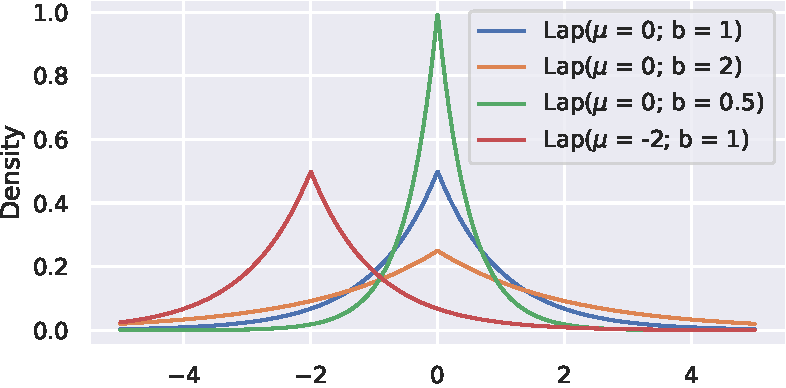
\includegraphics[width=0.8\linewidth]{img/laplace-distributions.pdf}
\caption{Laplace PDF (probability density function)}
\end{figure}
$$
\textrm{Lap}(x; \mu, b) = \frac{1}{2b} \exp \left( - \frac{\abs{x - \mu}}{b}  \right)
$$

%\begin{tikzpicture}[overlay, remember picture]
%\node at (current page.north east)[ref] {
%\fullcite{Voigt.Bussche.2017} \par};
%\end{tikzpicture}
\end{frame}





\begin{frame}{How to choose the parameters?}

Location and scale

-- Location: the true value

-- Scale?

Let's pick $b = 1$ just for lack of better ideas :)

%\begin{tikzpicture}[overlay, remember picture]
%\node at (current page.north east)[ref] {
%\fullcite{Voigt.Bussche.2017} \par};
%\end{tikzpicture}
\end{frame}



\begin{frame}{It's all nice and random, but what does it give us?}

Query: How many persons in the database take illegal drugs?

\begin{table}
\footnotesize
\begin{tabular}{lrrr} \toprule
Name & Hospitalized in year & Age & Illegal drug use \\ \midrule
Alice & 2024 & 32 & yes \\
Bob & 2020 & 21 & no \\
Charlie & 2023 & 45 & no \\
$\ldots$ & & & \\
Xander & 2020 & 31 & yes \\ \bottomrule
\end{tabular}
\caption{Database $D$, including Alice}
\end{table}


Assume that the true answer is 51

%\begin{tikzpicture}[overlay, remember picture]
%\node at (current page.north east)[ref] {
%\fullcite{Voigt.Bussche.2017} \par};
%\end{tikzpicture}
\end{frame}


\begin{frame}{It's all nice and random, but what does it give us?}

What if Alice decided \textbf{not to be part of the data}?

-- She has the right to decide about her privacy, GDPR, etc.

\begin{table}
\footnotesize
\begin{tabular}{lrrr} \toprule
Name & Hospitalized in year & Age & Illegal drug use \\ \midrule
Bob & 2020 & 21 & no \\
Charlie & 2023 & 45 & no \\
$\ldots$ & & & \\
Xander & 2020 & 31 & yes \\ \bottomrule
\end{tabular}
\caption{Database $D'$, \textbf{excluding} Alice}
\end{table}

The true answer to the query would be now 50


%\begin{tikzpicture}[overlay, remember picture]
%\node at (current page.north east)[ref] {
%\fullcite{Voigt.Bussche.2017} \par};
%\end{tikzpicture}
\end{frame}


\begin{frame}{We have two databases: With and without Alice}

Privatize for $D$ (with Alice), true answer is 51
$$
Y \sim \frac{1}{2b} \exp \left( \frac{-\abs{x - 51}}{b} \right) = \frac{1}{2} \exp \left( -\abs{x - 51} \right) 
$$

\begin{figure}
\centering
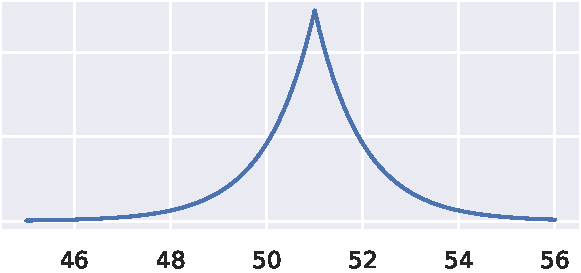
\includegraphics[width=0.7\linewidth]{img/laplace-density1.pdf}
\caption{Laplace density, $\mu = 51, b = 1$}
\end{figure}

%\begin{tikzpicture}[overlay, remember picture]
%\node at (current page.north east)[ref] {
%\fullcite{Voigt.Bussche.2017} \par};
%\end{tikzpicture}
\end{frame}



\begin{frame}{Now without Alice}


Privatize for $D'$ (without Alice), true answer is 50
$$
Y' \sim \frac{1}{2b} \exp \left( \frac{-\abs{x - 50}}{b} \right) = \frac{1}{2} \exp \left( -\abs{x - 50} \right) 
$$


\begin{figure}
\centering
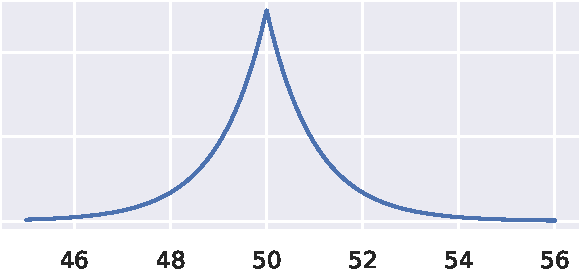
\includegraphics[width=0.7\linewidth]{img/laplace-density2.pdf}
\caption{Laplace density, $\mu = 50, b = 1$}
\end{figure}

%\begin{tikzpicture}[overlay, remember picture]
%\node at (current page.north east)[ref] {
%\fullcite{Voigt.Bussche.2017} \par};
%\end{tikzpicture}
\end{frame}

\begin{frame}{Both variables in one plot}
$
Y \sim  \frac{1}{2} \exp \left( -\abs{x - 51} \right) \qquad
Y' \sim \frac{1}{2} \exp \left( -\abs{x - 50} \right) 
$

\begin{figure}
\centering
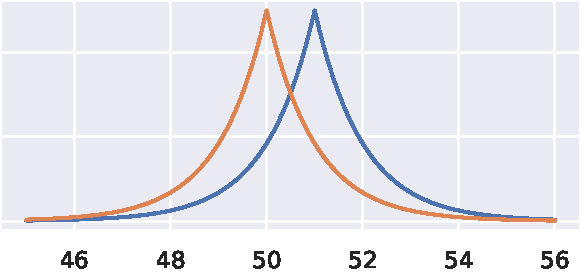
\includegraphics[width=0.6\linewidth]{img/laplace-02.pdf}
\caption{Blue = with Alice, red = without Alice}
\end{figure}

Now observe a particular value $y \in \mathbb{R}$, for example 52

-- Was it sampled from $Y$ or from $Y'$?

%\begin{tikzpicture}[overlay, remember picture]
%\node at (current page.north east)[ref] {
%\fullcite{Voigt.Bussche.2017} \par};
%\end{tikzpicture}
\end{frame}


\begin{frame}{If we observed 52, was it sampled from $Y$ or from $Y'$?}

We cannot really tell!

But we can compare probabilities of this event\footnote{We must compare densities, so our math will not break}

$
\Pr[Y = 52] = \frac{1}{2} \exp \left( -\abs{52 - 51} \right) = 0.5 \exp(-1)
$
$
\Pr[Y' = 52] = \frac{1}{2} \exp \left( -\abs{52 - 50} \right) = 0.5 \exp(-2)
$

How much more likely from $Y$?
$
\frac{\Pr[Y = 52]}{\Pr[Y' = 52]}
= \frac{0.5 \exp(-1)}{0.5 \exp(-2)} = \exp(-1)\exp(2) = \exp(1) = 2.718
$

How much more likely from $Y'$?
$
\frac{\Pr[Y' = 52]}{\Pr[Y = 52]}
= \frac{0.5 \exp(-2)}{0.5 \exp(-1)} = \exp(-1) = 0.367
$

%\begin{tikzpicture}[overlay, remember picture]
%\node at (current page.north east)[ref] {
%\fullcite{Voigt.Bussche.2017} \par};
%\end{tikzpicture}
\end{frame}



\begin{frame}{Both variables in one plot}
$
Y \sim  \frac{1}{2} \exp \left(- \abs{x - 51} \right) \qquad
Y' \sim \frac{1}{2} \exp \left(- \abs{x - 50} \right) 
$

\begin{figure}
\centering
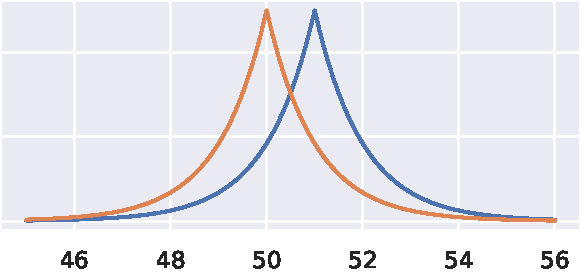
\includegraphics[width=0.6\linewidth]{img/laplace-02.pdf}
\caption{Blue = with Alice, red = without Alice}
\end{figure}

Now observe a particular value $y \in \mathbb{R}$, for example 50

-- Was it sampled from $Y$ or from $Y'$?

%\begin{tikzpicture}[overlay, remember picture]
%\node at (current page.north east)[ref] {
%\fullcite{Voigt.Bussche.2017} \par};
%\end{tikzpicture}
\end{frame}



\begin{frame}{If we observed 50, was it sampled from $Y$ or from $Y'$?}

$
\Pr[Y = 50] = \frac{1}{2} \exp \left(- \abs{50 - 51} \right) = 0.5 \exp(-1)
$
$
\Pr[Y' = 50] = \frac{1}{2} \exp \left(- \abs{50 - 50} \right) = 0.5 \exp(0)
$

How much more likely from $Y$?
$
\frac{\Pr[Y = 50]}{\Pr[Y' = 50]}
= \frac{0.5 \exp(-1)}{0.5 \exp(0)} = \exp(-1) = 0.367
$

How much more likely from $Y'$?
$
\frac{\Pr[Y' = 50]}{\Pr[Y = 50]}
= \frac{0.5 \exp(0)}{0.5 \exp(-1)} = \exp(1) = 2.718
$

It seems like the odds ratio is bounded from above...

%\begin{tikzpicture}[overlay, remember picture]
%\node at (current page.north east)[ref] {
%\fullcite{Voigt.Bussche.2017} \par};
%\end{tikzpicture}
\end{frame}

\begin{frame}{Can we generalize it for any observed $x$?}

\begin{figure}
\centering
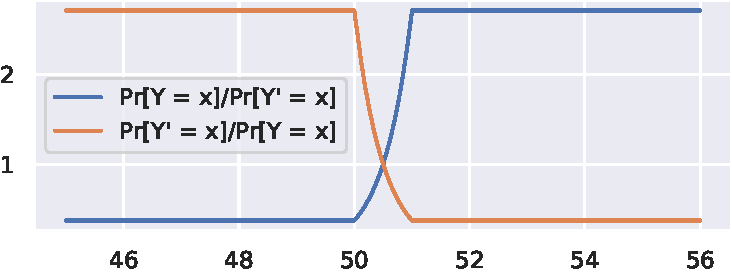
\includegraphics[width=0.8\linewidth]{img/laplace-03.pdf}
\end{figure}

Seems like the maximum we can get is $2.718 = e = \exp(1)$

%\begin{tikzpicture}[overlay, remember picture]
%\node at (current page.north east)[ref] {
%\fullcite{Voigt.Bussche.2017} \par};
%\end{tikzpicture}
\end{frame}


\begin{frame}{Let's try to prove it}

We need triangle inequality for absolute values:\footnote{Homework: Prove it! $x, y \in \mathbb{R}$}
$\abs{x} - \abs{y} \leq \abs{x - y}$

$$
\begin{aligned}
\frac{\Pr[Y = x]}{\Pr[Y' = x]} =
\frac{
\frac{1}{2} \exp \left(- \abs{x - 51} \right)
}{
\frac{1}{2} \exp \left(-\abs{x - 50} \right) 
}
&= \exp ( \abs{x - 50} - \abs{x - 51} ) \\
&\leq \exp ( \abs{(x - 50) - (x - 51)} ) \\
&= \exp ( \abs{x - 50 - x + 51} ) \\
&= \exp ( \abs{1}) = \exp(1) \\
\end{aligned}
$$

\end{frame}


\begin{frame}{Let's try to prove it (part 2)}


$$
\begin{aligned}
\frac{\Pr[Y' = x]}{\Pr[Y = x]} =
\frac{
	\frac{1}{2} \exp \left( - \abs{x - 50} \right)
}{
	\frac{1}{2} \exp \left( - \abs{x - 51} \right) 
}
&= \exp ( \abs{x - 51} - \abs{x - 50} ) \\
&\leq \exp ( \abs{(x - 51) - (x - 50)} ) \\
&= \exp ( \abs{x - 51 - x + 50} ) \\
&= \exp (\abs{-1}) = \exp(1)
\end{aligned}
$$



%\begin{tikzpicture}[overlay, remember picture]
%\node at (current page.north east)[ref] {
%\fullcite{Voigt.Bussche.2017} \par};
%\end{tikzpicture}
\end{frame}


\begin{frame}{What does that mean?}
\begin{figure}
\centering
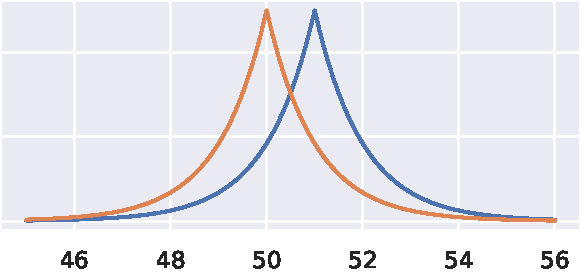
\includegraphics[width=0.4\linewidth]{img/laplace-02.pdf}
\caption{Blue = with Alice, red = without Alice, $Y \sim  \frac{1}{2} \exp \left(- \abs{x - 51} \right) \qquad
Y' \sim \frac{1}{2} \exp \left(- \abs{x - 50} \right)$}
\end{figure}

$
\frac{\Pr[Y = x]}{\Pr[Y' = x]} \leq \exp(1) \qquad
\frac{\Pr[Y' = x]}{\Pr[Y = x]} \leq \exp(1)
$


No matter what value we get after privatizing the counting query -- we can only get some limited "information" about whether it came from $Y$ or $Y'$.



%\begin{tikzpicture}[overlay, remember picture]
%\node at (current page.north east)[ref] {
%\fullcite{Voigt.Bussche.2017} \par};
%\end{tikzpicture}
\end{frame}





\begin{frame}{What if the true answer would be the same for $D$ and $D'$?}

Alice did not take drugs
$
Y \sim  \frac{1}{2} \exp \left(- \abs{x - 50} \right) \qquad
Y' \sim \frac{1}{2} \exp \left(- \abs{x - 50} \right) 
$

\begin{figure}
\centering
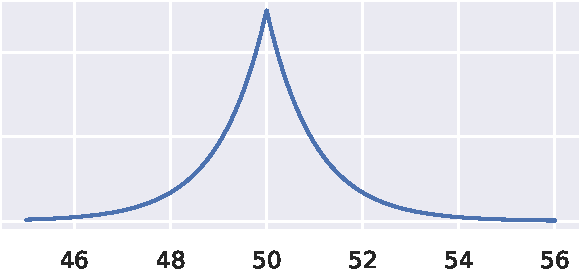
\includegraphics[width=0.4\linewidth]{img/laplace-density2.pdf}
\caption{Both have the same distribution}
\end{figure}

$
\frac{\Pr[Y = x]}{\Pr[Y' = x]} = 1 \leq \exp(1) \qquad
\frac{\Pr[Y' = x]}{\Pr[Y = x]} = 1 \leq \exp(1)
$

So the maximum "loss" only when the presence of Alice changes the query output

%\begin{tikzpicture}[overlay, remember picture]
%\node at (current page.north east)[ref] {
%\fullcite{Voigt.Bussche.2017} \par};
%\end{tikzpicture}
\end{frame}


\begin{frame}{What if the true answer would be 22?}

Alice did not take drugs
$
Y \sim  \frac{1}{2} \exp \left(- \abs{x - 22} \right) \qquad
Y' \sim \frac{1}{2} \exp \left( -\abs{x - 22} \right) 
$

-- bounded by 1 as in the previous slide 

Alice did take drugs

$Y \sim  \frac{1}{2} \exp \left(- \abs{x - 23} \right) \qquad
Y' \sim \frac{1}{2} \exp \left(- \abs{x - 22} \right)$

-- our general proof still holds!
$
\frac{\Pr[Y = x]}{\Pr[Y' = x]} \leq \exp(1) \qquad
\frac{\Pr[Y' = x]}{\Pr[Y = x]} \leq \exp(1)
$

%\begin{tikzpicture}[overlay, remember picture]
%\node at (current page.north east)[ref] {
%\fullcite{Voigt.Bussche.2017} \par};
%\end{tikzpicture}
\end{frame}


\begin{frame}{Summary}

Four counting queries, the maximum difference of the query result is 1 (when a particular person is not in the dataset)

We used scale $b = 1$ for the Laplace distribution, which gives us upper bound on privacy loss

$
\frac{\Pr[Y = x]}{\Pr[Y' = x]} \leq \exp(1) \qquad
\frac{\Pr[Y' = x]}{\Pr[Y = x]} \leq \exp(1)
$

%\begin{tikzpicture}[overlay, remember picture]
%\node at (current page.north east)[ref] {
%\fullcite{Voigt.Bussche.2017} \par};
%\end{tikzpicture}
\end{frame}



\begin{frame}{License and credits}

	\begin{columns}
		\begin{column}{0.7\textwidth}
			Licensed under Creative Commons Attribution-ShareAlike 4.0 International (CC BY-SA 4.0)
		\end{column}
		\begin{column}{0.2\textwidth}
			
\includegraphics[width=0.9\linewidth]{img/cc-by-sa-icon.pdf}
		\end{column}
	\end{columns}
	
	\bigskip
	
	Credits
	
	\begin{scriptsize}
		
		Ivan Habernal
		
		Content from ACL Anthology papers licensed under CC-BY \url{https://www.aclweb.org/anthology}
		
		Partly inspired by lectures from Antti Honkela, Aurélien Bellet, Gautam Kamath
	
	\end{scriptsize}
	
\end{frame}



\end{document}

